%\title{Overleaf Memo Template}
% Using the texMemo package by Rob Oakes
\documentclass[letter,12pt]{texMemo}
\usepackage[english]{babel}
\usepackage{color, listings, graphicx, float, booktabs, multirow, outlines, changepage, fancybox, enumitem}
\pagenumbering{gobble}

%% Edit the header section here. To include your
%% own logo, upload a file via the files menu.
\memoto{Whom It May Concern}
\memofrom{Alejandro Andrade, Kyle Salitrik}
\memosubject{Nurse Scheduling Database Final Design and Queries}
\memodate{\today}
%\logo{
\includegraphics[width=0.3\textwidth]{Overleaf-logo.jpg}}
\graphicspath{{./figures/}}

\definecolor{codegreen}{rgb}{0,0.6,0}
\definecolor{codegray}{rgb}{0.5,0.5,0.5}
\definecolor{codepurple}{rgb}{0.58,0,0.82}
\definecolor{backcolour}{rgb}{0.97,0.97,0.97}
 
\lstdefinestyle{mystyle}{
    %backgroundcolor=\color{backcolour},   
    basicstyle=\footnotesize,
    breakatwhitespace=false,         
    breaklines=true,                 
    captionpos=b,                    
    keepspaces=true,                 
%    numbers=left,                    
%    numbersep=5pt,                  
    showspaces=false,                
    showstringspaces=false,
    showtabs=false,                  
    tabsize=2
}

\lstdefinestyle{smallstyle}{
    %backgroundcolor=\color{backcolour},   
    basicstyle=\scriptsize,
    breakatwhitespace=false,         
    breaklines=true,                 
    captionpos=b,                    
    keepspaces=true,                 
%    numbers=left,                    
%    numbersep=5pt,                  
    showspaces=false,                
    showstringspaces=false,
    showtabs=false,                  
    tabsize=2
}
 
\lstset{style=mystyle}

\def\changemargin#1#2{\list{}{\rightmargin#2\leftmargin#1}\item[]}
\let\endchangemargin=\endlist 

\makeatletter
\newenvironment{CenteredBox}{% 
\begin{Sbox}}{% Save the content in a box
\end{Sbox}\centerline{\parbox{\wd\@Sbox}{\TheSbox}}}% And output it centered
\makeatother

\begin{document}
\maketitle
The purpose of the following document is to explain in depth a database for a nursing care assistance hospital or clinic. Such database was created to solve the problem of scheduling each shift and combining the available resources to meet the working constraints of each nurse.

The database model and the select examples give an overview of the relationship and capabilities of the data. It is important that data can get increasingly big and processing the select queries can exponentially increase in run time. Thus, this document also explains how the database is internally optimized to avoid long run time processing through indexing techniques. The data model that will be referenced throughout the document is attached at the end of the document.
\section*{Table Specifications}
This section contains the specifications for each table used in the relational model.
	\subsection*{Address}
		The address table contains the information for an address, with each address being linked to an employee by their employee ID. This allows the database to handle employees with multiple addresses without wasting space by having multiple address fields per employee.
		\lstinputlisting[language=]{./code/table_address.txt}
	\newpage
	\subsection*{Certification}
		Each certification is linked to a role by the role ID and an employee by their employee ID. This implementation allows an employee to have multiple registered certifications.
		\lstinputlisting[language=]{./code/table_certification.txt}
	\subsection*{Role}
		The role table contains the description of each role (RN, LPN, etc) in order to save storage space by preventing repeated copies of the data.
		\lstinputlisting[language=]{./code/table_role.txt}
	\subsection*{Department}
		The department table contains the department name and number of beds as well as the maximum and minimum amount of staff necessary.
		\lstinputlisting[language=]{./code/table_department.txt}
	\newpage
	\subsection*{Department Need}
		The department need table is linked to the week, day, shift time, department, and roles by their respective IDs. A single department need record contains the role and number of personnel needed for a particular shift on a particular day.
		\lstinputlisting[language=]{./code/table_department_need.txt}
	\subsection*{Employee}
		The employee table contains personal and financial information for each employee. The home department of the employee may be filled out, if applicable, via a foreign key to the department table.
		\lstinputlisting[language=]{./code/table_employee.txt}
	\newpage	
	\subsection*{Shift}
		The shift table contains entries for a specific shift for a specific employee on a specific day. The table is linked to the employee, department, shift time, week, day, and shift status tables by their respective foreign keys. The pay modifier may be adjusted to increase the employee's shift pay if they are called in or work a special shift such as a holiday.
		\lstinputlisting[language=]{./code/table_shift.txt}
	\subsection*{Shift Status}
		The shift status table contains information with common notes for a shift, such as someone calling off, requesting the shift off, requesting to be staffed for the shift or being called in.
		\lstinputlisting[language=]{./code/table_shift_status.txt}
	\subsection*{Shift Time}
		The shift times table contains the hospital's current shift schedules.
		\lstinputlisting[language=]{./code/table_shift_time.txt}
	\newpage	
	\subsection*{Week}
		The week table was created to easily access shifts by week, as it serves only to be used in the shift as a foreign key for this purpose.
		\lstinputlisting[language=]{./code/table_week.txt}
	\subsection*{Weekday}
		The weekday table contains the days of the week as text in order to save on data storage and time costs of re-writing the names of each day repeatedly.
		\lstinputlisting[language=]{./code/table_weekday.txt}

\newpage
\section*{Desired Queries}
Within this section all queries are explained, the MySQL query itself is given, indexing is discussed and one weeks worth of sample data is provided. If the sample data exceeded 100 lines, the result was truncated to 100 lines for brevity.
%---------------------------------------------
\subsection*{Query 1}
The first query is designed to return a single employee's schedule for any given 6 week period. It shall return the week start date, day of week, shift, department, and role for the employee. The input parameters to the query are the start week, end week, and ID of the employee in question.
\subsubsection*{MySQL Query}
	\lstinputlisting[language=]{./code/query1.txt}
\begin{figure}[H]
	\centering
	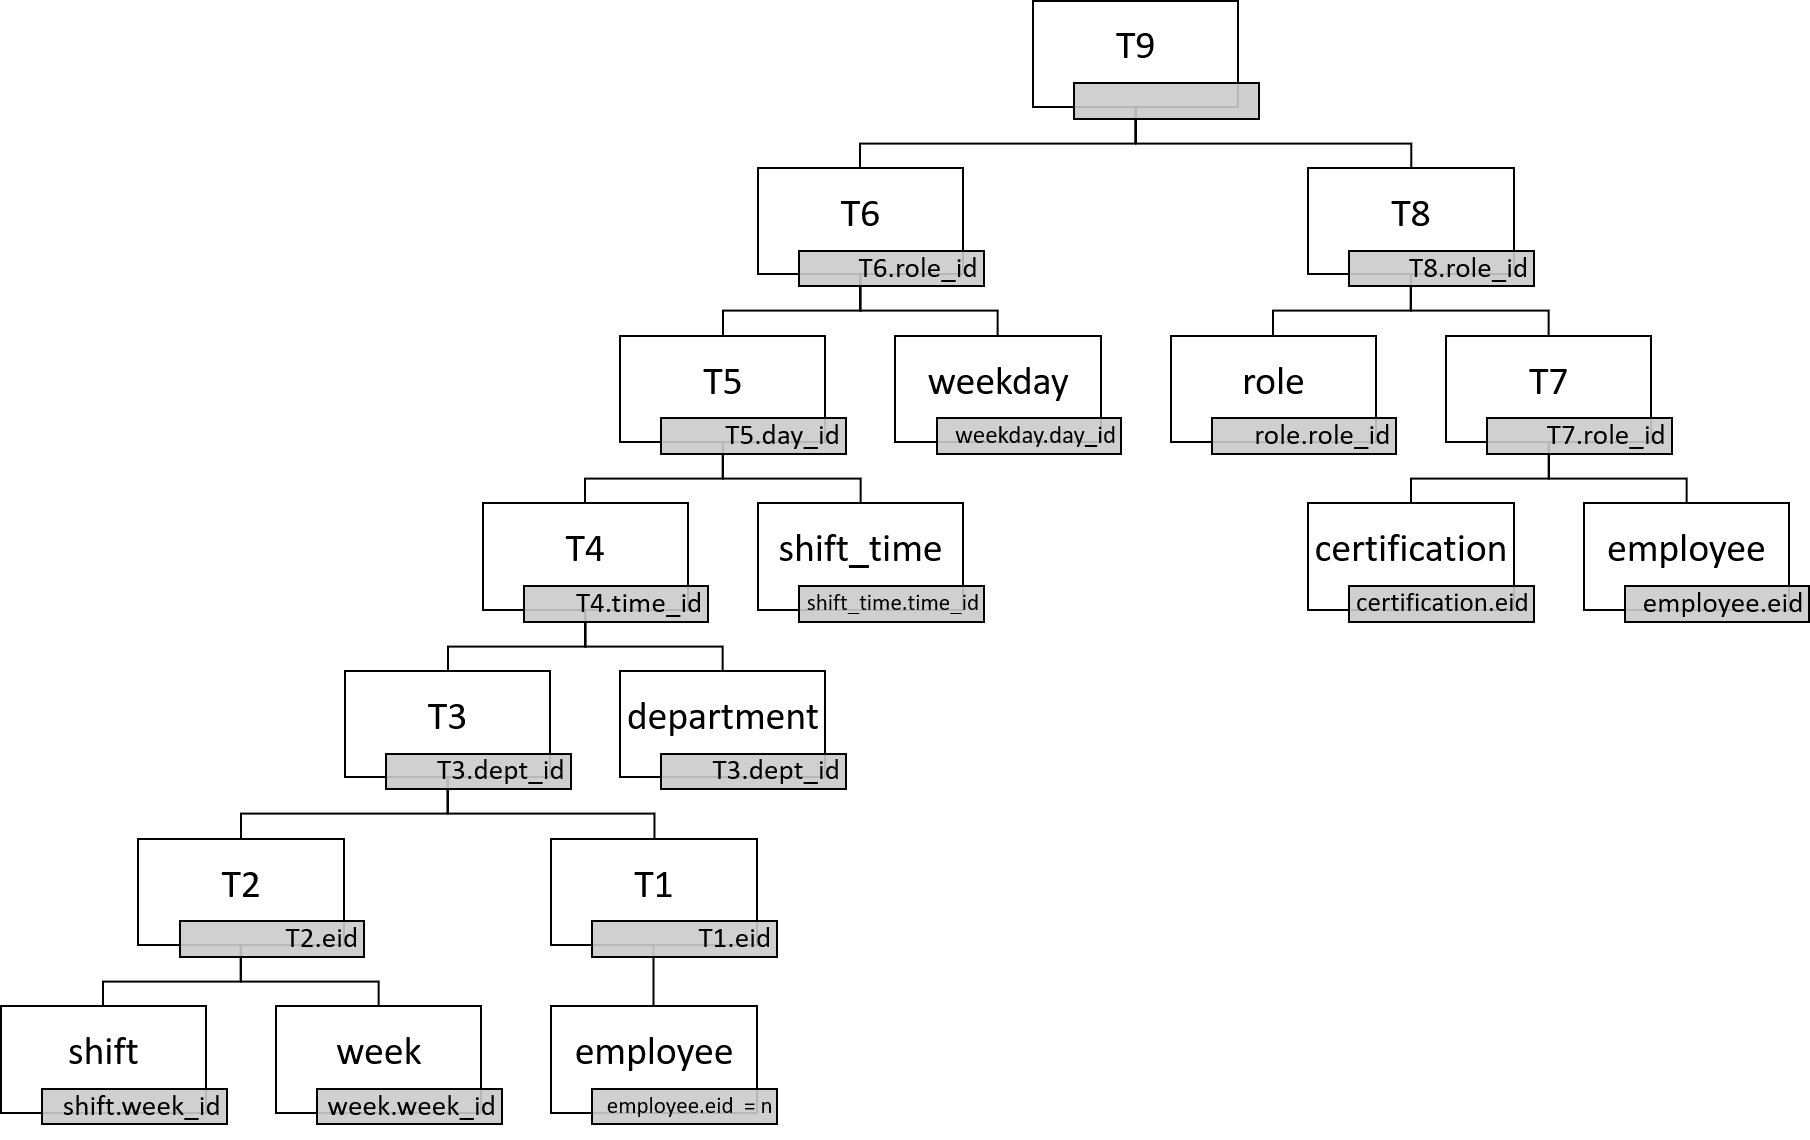
\includegraphics[width=\textwidth]{query1.png}
\end{figure}
For the first query, the best table to index is Shift on shift\_id and week\_id. This index is chosen because the shift table will be the second largest table in the database (only department\_need will be larger) and the ability to quickly find the desired weeks for the employee's schedule. This will narrow down the number of records to a maximum of 30 times the number of employees, and has the following costs.
\begin{itemize}[noitemsep,nolistsep]
	\item Week Between Dates: T0 = O(W)
	\item Shift-Week Join: T1 = O(S*T0)
	\item Employee Equal to N: O(E)
	\item T1-Emp Join: T2 = O(SW) because there will only be 1 employee
	\item T2-Department Join: T3 = O(T2 D)
	\item T3-Time Join: T4 = O(T3 Time)
	\item T4-Weekday Join: T4 = O(T4 Weekday)
	\item Certification-Employee Join: T5 = O(C * E)
	\item T5-Role Join: T6 = O(T5 R)
	\item T4-T6 Join: T7 = O(T4 * T6)
\end{itemize}

\begin{figure}[H]
	\centering
	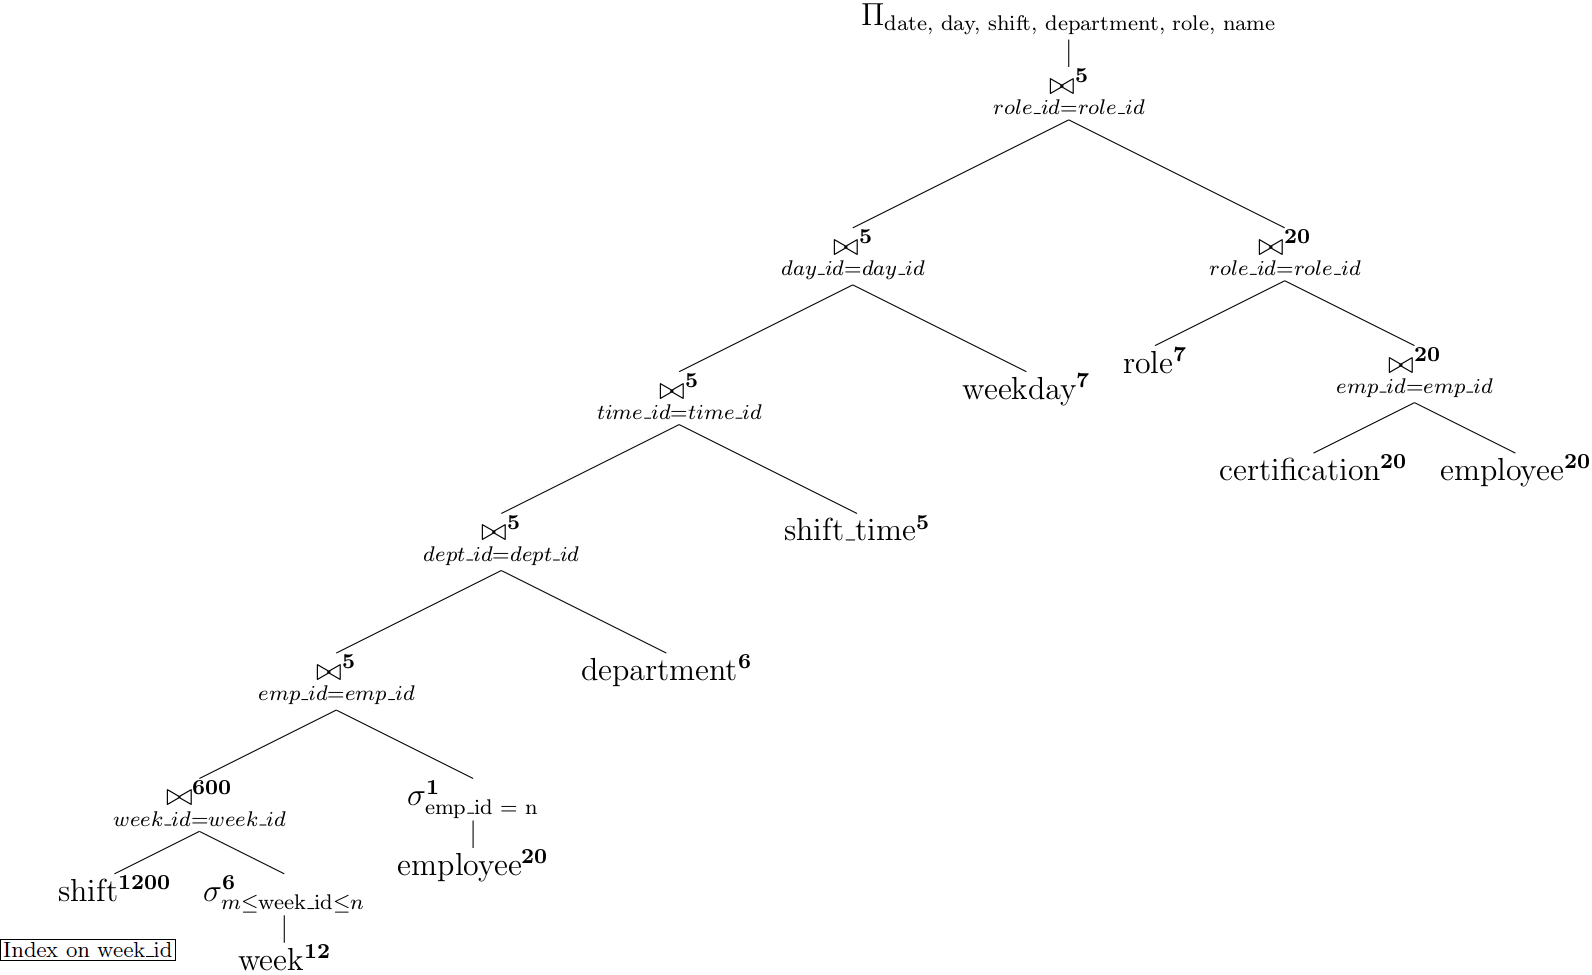
\includegraphics[width=\textwidth]{query1_indexed.png}
\end{figure}
Using the indexes stated has the following effect on the query execution time:
\begin{itemize}[noitemsep,nolistsep]
	\item Week Between Dates: T0 = O(W)
	\item Shift-Week Join: T1 = O(S*T0) $\rightarrow$ O(S*log T0)
	\item Employee Equal to N: O(E)
	\item T1-Emp Join: T2 = O(SW) because there will only be 1 employee
	\item T2-Department Join: T3 = O(T2 D)
	\item T3-Time Join: T4 = O(T3 Time)
	\item T4-Weekday Join: T4 = O(T4 Weekday)
	\item Certification-Employee Join: T5 = O(C * E)
	\item T5-Role Join: T6 = O(T5 R)
	\item T4-T6 Join: T7 = O(T4 * T6)
\end{itemize}


\vspace{1em}
\subsubsection*{Example Data}
\lstset{style=smallstyle}
	\begin{center}
		\lstinputlisting[language=]{./code/query1_data.txt}
	\end{center}
\lstset{style=mystyle}

%---------------------------------------------
\subsection*{Query 2}
Query 2 returns a department's need for a single week including the week's start date, day of week, shift start time, shift end time, and needs per role per shift. The query can be tuned by changing the department ID and week ID.

\subsubsection*{MySQL Query}
	\lstinputlisting[language=]{./code/query2.txt}
\begin{figure}[H]
	\centering
	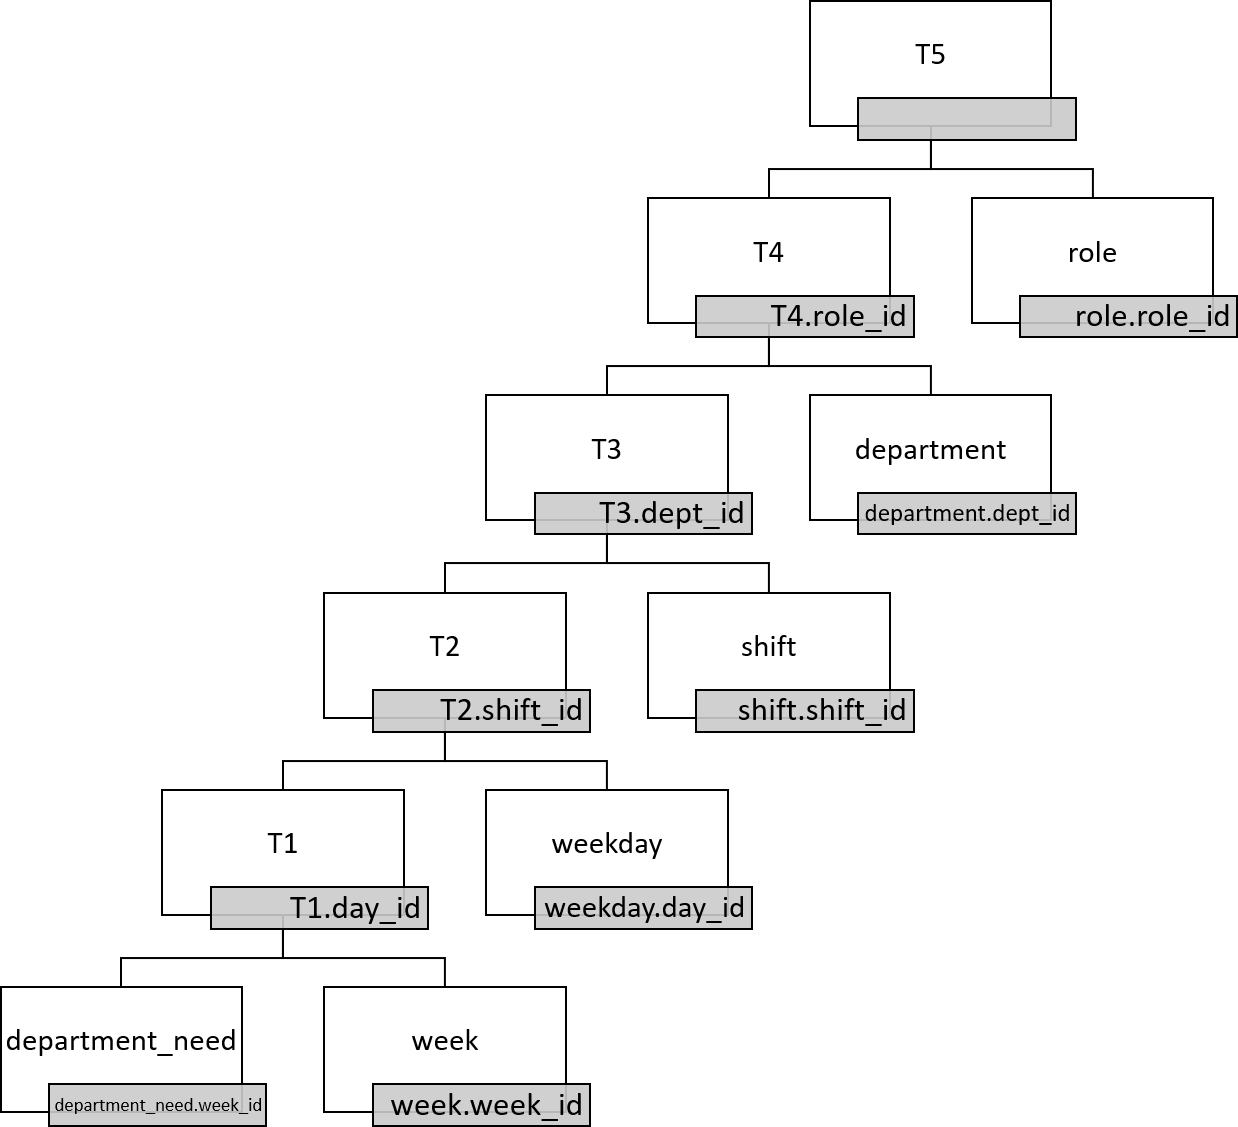
\includegraphics[width=.75\textwidth]{query2.png}
\end{figure}
For the second query the process is much similar to query one. The difference is that the table that is getting joined for the following select query is the departments table. Following the above principle one can optimize the run-time of the query by indexing shifts on shift\_id and department\_id to optimize the given big-O runtimes.
\begin{itemize}[noitemsep,nolistsep]
	\item Week Equals: T0 = O(W)
	\item Need-Week Join: T1 = O(N*T0)
	\item T1-Weekday: T2 = O(T1 Weekday)
	\item T2-Shift: T3 = O(T2 S)
	\item T3-Department: T4 = O(T3 D)
	\item T4-Role: T5 = O(T4 R)
\end{itemize}

\begin{figure}[H]
	\centering
	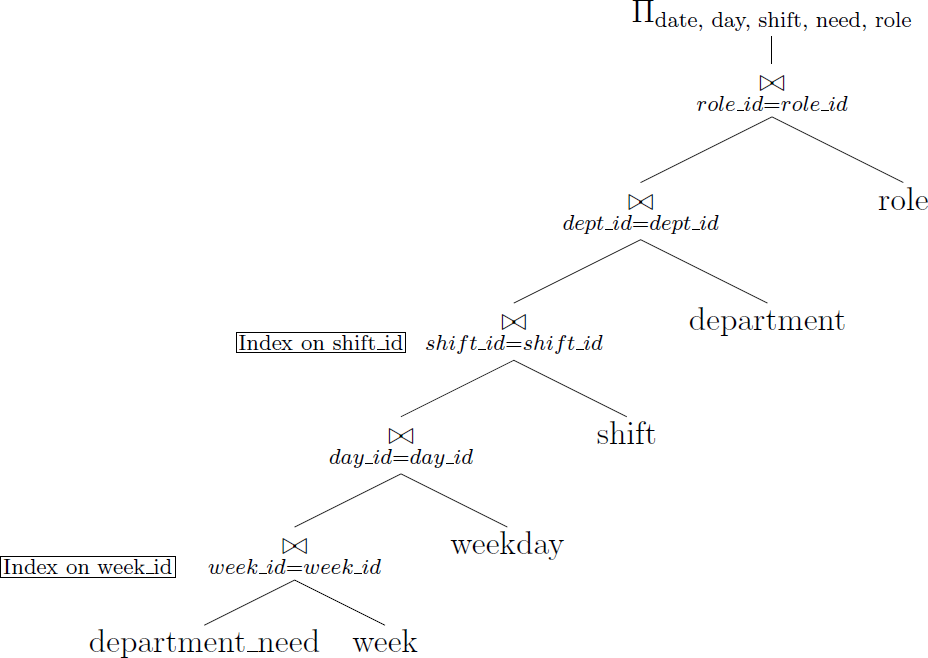
\includegraphics[width=.75\textwidth]{query2_indexed.png}
\end{figure}
Creating the indexing described above yields log(N) access for both the shifts and department tables, providing a significant speed up because these two tables will be the largest within the database. The optimized runtime changes are shown below:
\begin{itemize}[noitemsep,nolistsep]
	\item Need-Week Join: T1 = O(N*W) $\rightarrow$ O(log(N) * W)
	\item T1-Weekday: T2 = O(T1 Weekday)
	\item T2-Shift: T3 = O(T2 Shift) $\rightarrow$ O(T2 log(S))
	\item T3-Department: T4 = O(T3 D)
	\item T4-Role: T5 = O(T4 R)
\end{itemize}

\vspace{1em}
\subsubsection*{Example Data}
\lstset{style=smallstyle}
	\begin{center}
		\lstinputlisting[language=]{./code/query2_data.txt}
	\end{center}
\lstset{style=mystyle}

%---------------------------------------------
\subsection*{Query 3}
Query 3 will give a single department's schedule for a specified week, ordered by the employee's names. Included information shall contain the start date of the week, the day of the week, shift start and end times, the employee's name, and their phone number. The department and week ID values will need to be changed in order to get the desired data.\subsubsection*{MySQL Query}
	\lstinputlisting[language=]{./code/query3.txt}
\begin{figure}[H]
	\centering
	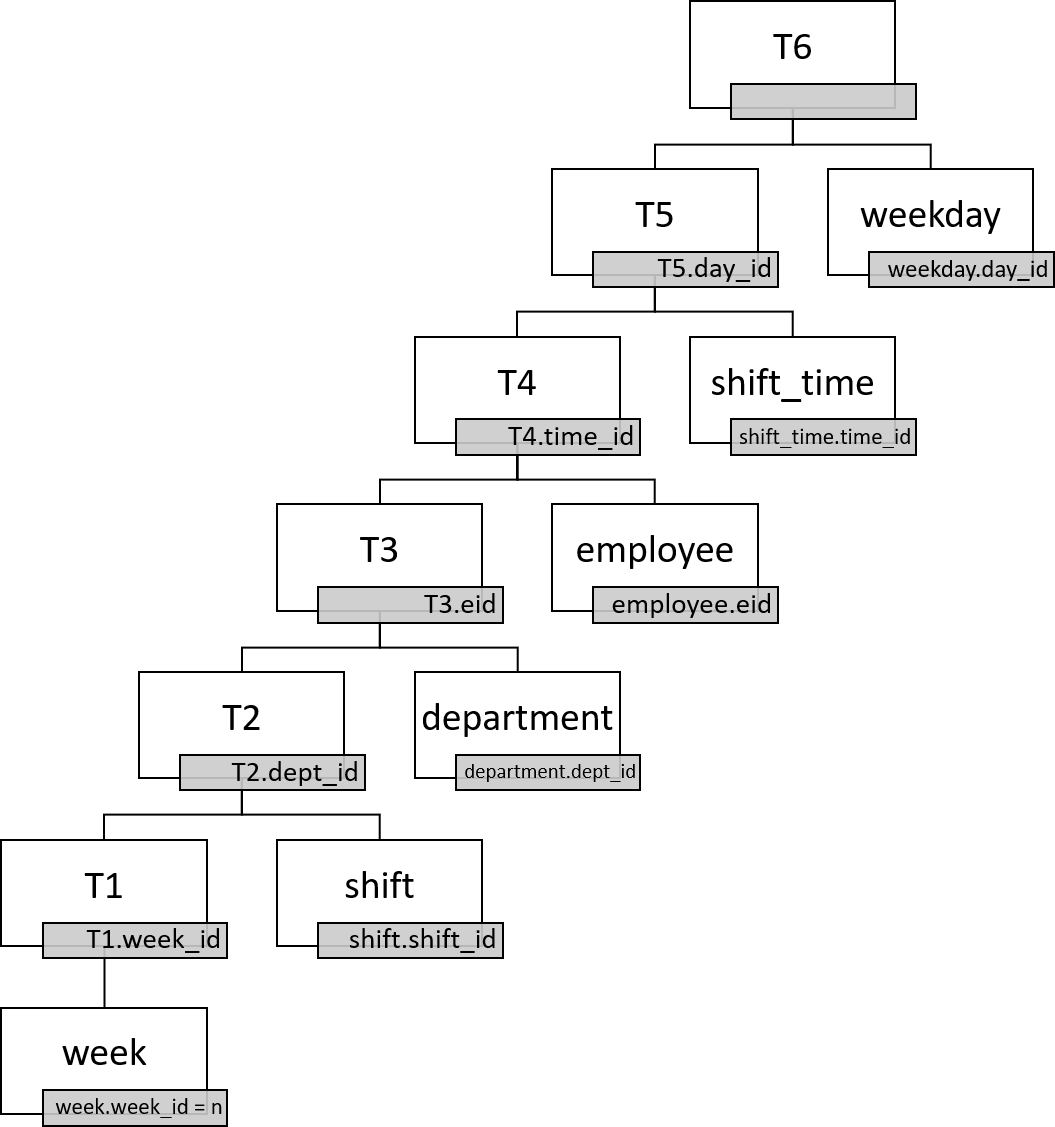
\includegraphics[width=.6\textwidth]{query3.png}
\end{figure}
For the third query a similar index scheme will be implemented on the shift table between the shift.week\_id and week.week\_id. The largest amount of comparisons occur during this table join. The time complexities for the joins are shown in the following list.
\begin{itemize}[noitemsep,nolistsep]
	\item Week = N: T1 = O(Week)
	\item T1-Shift Join: T2 = O(T1 S)
	\item T2-Department Join: T3 = O(T2 D)
	\item T3-Employee Join: T4 = O(T3 E)
	\item T4-Shift Time Join: T5 = O(T4 ST)
	\item T5-Weekday Join: T6 = O(T5 WD)
\end{itemize}

\begin{figure}[H]
	\centering
	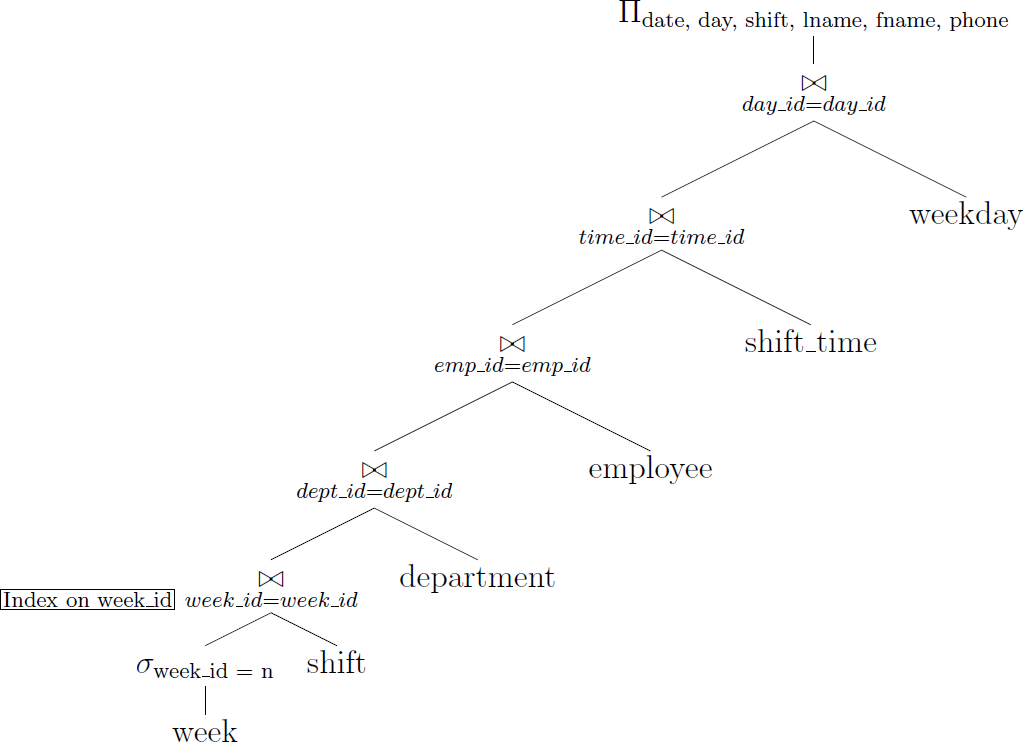
\includegraphics[width=.6\textwidth]{query3_indexed.png}
\end{figure}
The third query would experience the largest enhancement in the join between the tables from O(m*n) to O(log(m*n)+c) due to the ability to conduct a binary search on the values corresponding to the correct week ID for both tables and a linear search to find the beginning and end of that week.
\begin{itemize}[noitemsep,nolistsep]
	\item Week = N: T1 = O(Week)
	\item T1-Shift Join: T2 = O(T1 S) $\rightarrow$O(T1 log(S)) 
	\item T2-Department Join: T3 = O(T2 D)
	\item T3-Employee Join: T4 = O(T3 E)
	\item T4-Shift Time Join: T5 = O(T4 ST)
	\item T5-Weekday Join: T6 = O(T5 WD)
\end{itemize}

\vspace{1em}
\subsubsection*{Example Data}
\lstset{style=smallstyle}
	\begin{center}
		\lstinputlisting[language=]{./code/query3_data.txt}
	\end{center}
\lstset{style=mystyle}

%---------------------------------------------
\subsection*{Query 4}
Query 4 will return an employee's pay rate, department, shift start, and shift end times per shift when given a range of dates sorted by date and then shift start time. The total cost per shift shall be calculated by the data parser supplied by you.
\subsubsection*{MySQL Query}
	\lstinputlisting[language=]{./code/query4.txt}
\begin{figure}[H]
	\centering
	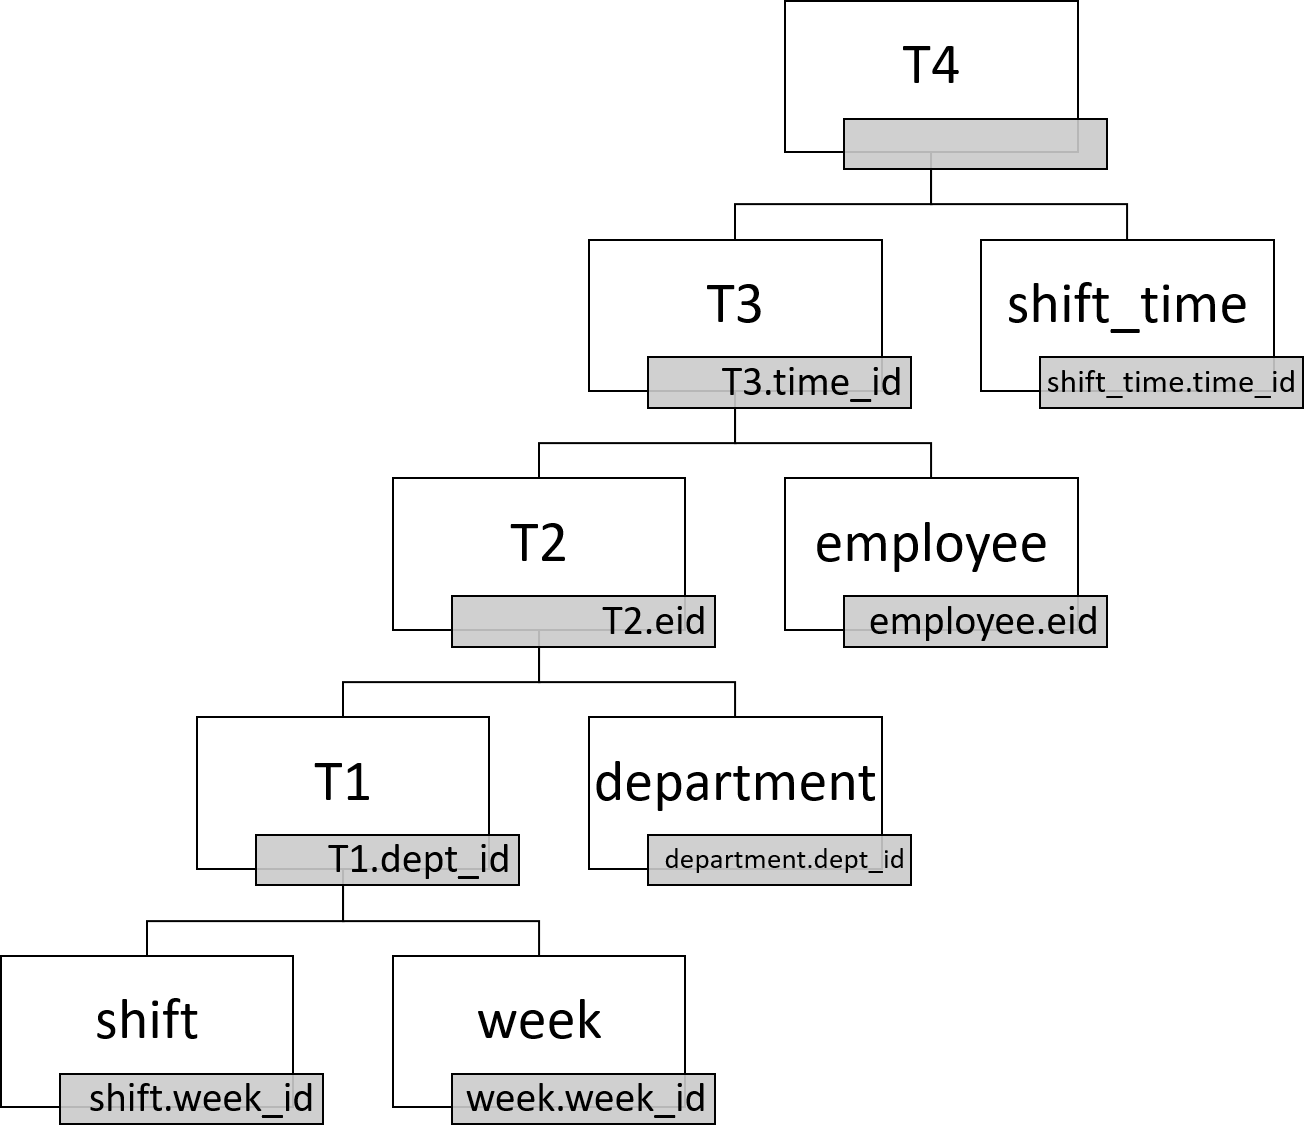
\includegraphics[width=.5\textwidth]{query4.png}
\end{figure}
Query 4 will also benefit from an index on the shift table between the shift.week\_id and week.week\_id. Again, the largest amount of comparisons occur during this table join. The time complexities for the joins are shown in the following list.
\begin{itemize}[noitemsep,nolistsep]
	\item Shift Between Days: T1 = O(S)
	\item T1-Week Join: T2 = O(T1 W) 
	\item T2-Department Join: T3 = O(T2 D)
	\item T3-Employee Join: T4 = O(T3 E)
	\item T4-Shift Time Join: T5 = O(T4 ST)
\end{itemize}

.\begin{figure}[H]
	\centering
	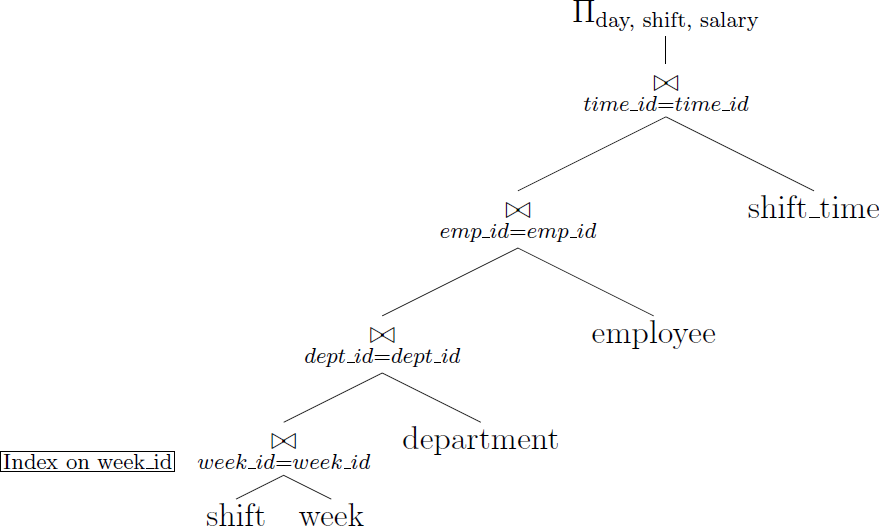
\includegraphics[width=.5\textwidth]{query4_indexed.png}
\end{figure}
For the fourth query, selecting the shifts between date ranges is the only step involving large amounts of data to compare. Indexing this first step would be the most beneficial to the query execution and would result in the new execution time below.
\begin{itemize}[noitemsep,nolistsep]
	\item Shift Between Days: T1 = O(S) $\rightarrow$ O(log(S))
	\item T1-Week Join: T2 = O(T1 W) 
	\item T2-Department Join: T3 = O(T2 D)
	\item T3-Employee Join: T4 = O(T3 E)
	\item T4-Shift Time Join: T5 = O(T4 ST)
\end{itemize}
\newpage
\subsubsection*{Example Data}
\lstset{style=smallstyle}
	\begin{center}
		\lstinputlisting[language=]{./code/query4_data.txt}
	\end{center}
\lstset{style=smallstyle}

\section*{Final Notes}
In closing, the supplied data model, table structures, and queries will return the data required by the specification documents. The indexes implemented should provide a considerable performance enhancement as the database grows. Output returned by the MySQL queries shall be parse-able by the program supplied by your company in order to create the desired output formats.

\newpage
\section*{Data Model}
\begin{figure}[H]
	\centering
	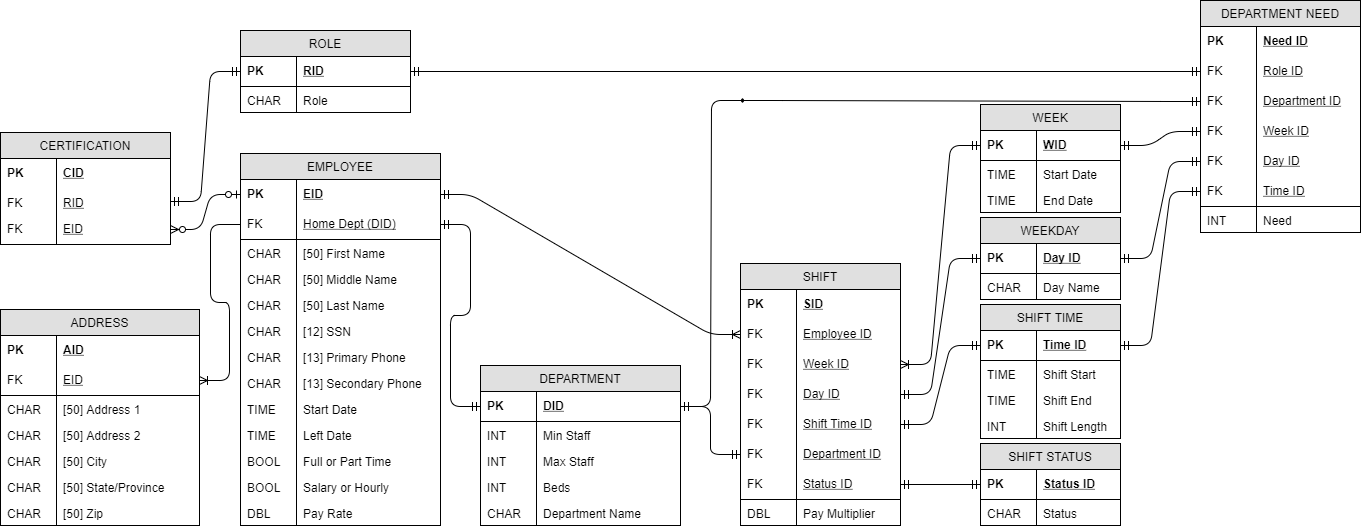
\includegraphics[angle=90, height=\textheight]{er_diag.png}
\end{figure}



%\bigskip{}\decorativeline\bigskip{}
%
%Sincerely,\\
%
%\quad Kyle Salitrik



\end{document}